% ====================================================================
%  Sistema Automatico de Clasificacion de Tomates -- Sistemas Embebidos II
%  Plantilla DCT - UCB San Pablo
%  VERSIÓN ACTUALIZADA: Servomotores MG996R + OLED
%  Editar SOLO este archivo (no tocar catolica_proyectos.cls)
% ====================================================================
\documentclass[12pt]{catolica_proyectos}
\addbibresource{bibliografia.bib}

% ---------------- PAQUETES ADICIONALES ----------------
\usepackage[T1]{fontenc}
\usepackage{float}
\usepackage{booktabs}
\usepackage{array}
\usepackage{siunitx}
\usepackage{listings}
\usepackage{tikz}
\usetikzlibrary{positioning,arrows.meta,shapes.geometric,automata,calc,fit,backgrounds}

% ---------------- COLORES ----------------
\definecolor{azulucb}{HTML}{1F4E79}
\definecolor{naranja}{HTML}{C55A11}
\definecolor{verdeok}{HTML}{2E7D32}
\definecolor{rojoerr}{HTML}{C0392B}
\definecolor{grisbox}{HTML}{F2F2F2}
\definecolor{griscmt}{HTML}{6A737D}

% ---------------- ESTILOS DE CODIGO ----------------
\lstset{
  basicstyle=\ttfamily\scriptsize,
  keywordstyle=\color{azulucb}\bfseries,
  commentstyle=\color{griscmt}\itshape,
  stringstyle=\color{verdeok},
  numbers=left, numberstyle=\tiny\color{griscmt}, numbersep=7pt,
  backgroundcolor=\color{grisbox},
  frame=single, rulecolor=\color{griscmt!50},
  breaklines=true, showstringspaces=false, tabsize=2,
  captionpos=b, extendedchars=true, inputencoding=utf8,
  literate=%
    {á}{{\'a}}1 {é}{{\'e}}1 {í}{{\'i}}1 {ó}{{\'o}}1 {ú}{{\'u}}1
    {Á}{{\'A}}1 {É}{{\'E}}1 {Í}{{\'I}}1 {Ó}{{\'O}}1 {Ú}{{\'U}}1
    {ñ}{{\~n}}1 {Ñ}{{\~N}}1 {ü}{{\"u}}1 {¿}{{?`}}1 {¡}{{!`}}1 {°}{{\textdegree}}1
}
\lstdefinestyle{C}{language=C}
\lstdefinestyle{py}{language=Python}
\lstdefinestyle{sh}{language=bash, numbers=none}

% ---------------- ESTILOS TikZ ----------------
\tikzset{
  bloque/.style={rectangle, rounded corners=2pt, draw=azulucb, very thick,
    fill=azulucb!8, align=center, minimum height=1cm, inner sep=5pt},
  cap/.style={rectangle, draw=griscmt, dashed, inner sep=8pt, rounded corners},
  flecha/.style={-{Stealth[length=2.5mm]}, thick},
  flechabi/.style={{Stealth[length=2.5mm]}-{Stealth[length=2.5mm]}, thick},
}

% ---------------- PLACEHOLDER PARA FOTOS REALES ----------------
\newcommand{\fotopendiente}[2][7cm]{%
  \fcolorbox{griscmt}{grisbox}{%
    \parbox[c][#1][c]{0.82\textwidth}{\centering\itshape\color{griscmt}
      [\,FOTOGRAFÍA REAL A INCORPORAR\,]\\[2pt] #2}}}

% ---------------- DATOS DEL PROYECTO ----------------
\titulo{Sistema Automático de Clasificación de Tomates mediante Visión Artificial y ESP32}
\materia{Sistemas Embebidos II}
\carrera{Mecatrónica}
\autor{Susann Baldiviezo C. \\ Alejandro Bejarano R. \\ Florencia Frigerio A. \\ Benjamín Soruco G.}
\docente{Msc. Ing. Alan Cornejo Q.}
\semestre{1/2026}

\begin{document}

\maketitle
\pagestyle{empty}
\tableofcontents
\newpage
\listoffigures
\newpage
\listoftables
\newpage

\pagenumbering{arabic}
\setcounter{page}{1}

% ====================================================================
\section{Descripción técnica-conceptual del proyecto a realizar}
% ====================================================================

El proyecto consiste en el diseño e implementación de un sistema automático de clasificación de tomates sobre una banda transportadora, que separa físicamente los frutos en buen estado de aquellos en estado de descomposición. La detección se realiza por visión artificial con OpenCV \cite{opencv2024,gonzalez2018dip}, mientras que toda la cadena de control, actuación, comunicación y monitoreo se resuelve con \textbf{sistemas embebidos basados en el microcontrolador ESP32} \cite{espressif2023trm}, que constituyen el núcleo de este documento.

El sistema se organiza en cuatro capas: (i)~\emph{adquisición}, con cámaras USB sobre la banda; (ii)~\emph{procesamiento}, en una PC que ejecuta el algoritmo de visión; (iii)~\emph{mensajería}, en una Raspberry Pi que actúa como \emph{broker} MQTT \cite{light2017mosquitto} y punto de acceso WiFi; y (iv)~\emph{actuación y monitoreo}, con dos ESP32 independientes: uno controla el motor de la banda y dos servomotores MG996R para desvío, y el otro es una consola portátil inalámbrica para el operario. La PC emite un veredicto binario por cada fruto (\texttt{aceptada} o \texttt{rechazada}) y lo publica en la red; los nodos embebidos reaccionan a ese mensaje en tiempo real.

El principal desafío técnico no está en la visión, sino en la \textbf{coordinación distribuida en tiempo real} entre nodos heterogéneos sin un cableado punto a punto: tres equipos (PC y dos ESP32) deben compartir estado de forma confiable, con baja latencia y de manera robusta ante desconexiones, sobre una red local que además debe funcionar \emph{sin acceso a Internet}. La propuesta de valor es ofrecer una solución de control de calidad poscosecha automatizada, portátil y de bajo costo, reproducible con componentes disponibles en el mercado local, orientada a pequeños productores (Sección~\ref{sec:tarija}).

En la Figura~\ref{fig:bloques} se presenta el diagrama en bloques del sistema. Se observa la separación en capas y, en particular, que la Raspberry Pi concentra la mensajería: ningún nodo se comunica directamente con otro, sino que todos publican y se suscriben a través del \emph{broker}, lo que desacopla a los dispositivos entre sí.

\begin{figure}[H]
  \centering
  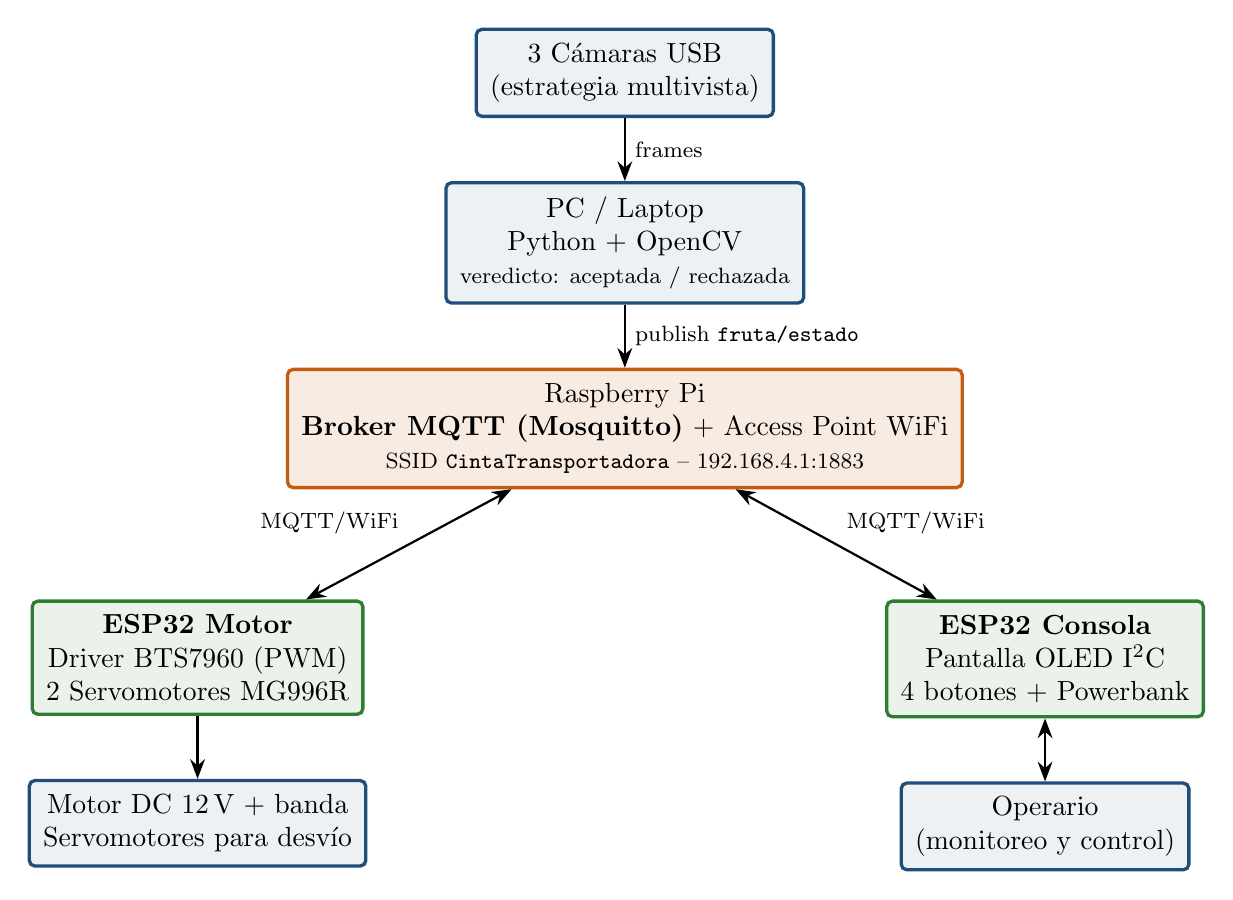
\begin{tikzpicture}[node distance=8mm and 14mm]
    % Capa entrada
    \node[bloque] (cam) {3 Cámaras USB\\(estrategia multivista)};
    % Capa procesamiento
    \node[bloque, below=of cam] (pc) {PC / Laptop\\Python + OpenCV\\\footnotesize veredicto: aceptada / rechazada};
    % Broker
    \node[bloque, fill=naranja!12, draw=naranja, below=of pc] (rpi)
      {Raspberry Pi\\\textbf{Broker MQTT (Mosquitto)} + Access Point WiFi\\\footnotesize SSID \texttt{CintaTransportadora} -- 192.168.4.1:1883};
    % Nodos embebidos
    \node[bloque, fill=verdeok!10, draw=verdeok, below left=14mm and -10mm of rpi] (m)
      {\textbf{ESP32 Motor}\\Driver BTS7960 (PWM)\\2 Servomotores MG996R};
    \node[bloque, fill=verdeok!10, draw=verdeok, below right=14mm and -10mm of rpi] (c)
      {\textbf{ESP32 Consola}\\Pantalla OLED I\textsuperscript{2}C\\4 botones + Powerbank};
    % Actuadores
    \node[bloque, below=of m] (act) {Motor DC 12\,V + banda\\Servomotores para desvío};
    \node[bloque, below=of c] (op) {Operario\\(monitoreo y control)};

    \draw[flecha] (cam) -- node[right,font=\footnotesize]{frames} (pc);
    \draw[flecha] (pc) -- node[right,font=\footnotesize]{publish \texttt{fruta/estado}} (rpi);
    \draw[flechabi] (rpi) -- node[above left,font=\footnotesize]{MQTT/WiFi} (m);
    \draw[flechabi] (rpi) -- node[above right,font=\footnotesize]{MQTT/WiFi} (c);
    \draw[flecha] (m) -- (act);
    \draw[flechabi] (c) -- (op);
  \end{tikzpicture}
  \caption{Diagrama en bloques del sistema actualizado con servomotores MG996R. La Raspberry Pi actúa como concentrador de mensajería (broker MQTT) y punto de acceso WiFi; los nodos se comunican de forma indirecta a través de tópicos.}
  \label{fig:bloques}
\end{figure}

% ====================================================================
\section{Propósito del proyecto}
% ====================================================================

El propósito es automatizar la clasificación poscosecha de tomate por estado de sanidad (sano vs. deteriorado), integrando visión artificial con un sistema embebido distribuido que controle los actuadores y permita la supervisión del operario en tiempo real. En concreto se busca:

\begin{itemize}
  \item Reducir la intervención humana en una tarea repetitiva y con alto margen de error visual, separando automáticamente el fruto deteriorado.
  \item Disminuir las pérdidas económicas asociadas a la comercialización de fruto en mal estado y al contagio de la podredumbre dentro del lote.
  \item Demostrar la viabilidad técnica de coordinar varios nodos embebidos ESP32 con una PC mediante un protocolo de mensajería liviano (MQTT) sobre una red WiFi local autónoma.
  \item Aplicar de forma integrada los contenidos de \emph{Sistemas Embebidos II}: GPIO, PWM, I\textsuperscript{2}C, conectividad WiFi, multitarea con FreeRTOS \cite{barry2016freertos} y control de actuadores de potencia.
\end{itemize}

Desde lo académico, el énfasis está en el \textbf{firmware embebido y la arquitectura de comunicaciones}; la visión artificial se trata como un módulo proveedor de veredictos cuya implementación interna es intercambiable.

% ====================================================================
\section{Alcance del proyecto}
% ====================================================================

El proyecto abarca el diseño, la construcción y la validación de un prototipo funcional. A continuación se delimita el alcance.

\subsection{Lo que el sistema SÍ contempla}
\begin{itemize}
  \item Firmware embebido para dos ESP32 desarrollado sobre ESP-IDF v5.x \cite{espressif2024idf}: control de motor por PWM, disparo de servomotores, lectura de botones y manejo de display OLED.
  \item Control de la banda transportadora mediante driver de potencia BTS7960 (puente H) \cite{infineon2013bts7960}.
  \item Expulsión física del fruto rechazado mediante dos servomotores MG996R acoplados mecánicamente con precisión angular de $\pm 5°$.
  \item Arquitectura de comunicaciones completa: red WiFi local con la Raspberry Pi como Access Point y \emph{broker} MQTT, definición de tópicos, calidad de servicio y secuencia de mensajes.
  \item Consola portátil (segunda ESP32) con pantalla OLED I\textsuperscript{2}C (128x64 px), cuatro botones, alimentada por \emph{powerbank} 12000\,mAh, para monitoreo y control inalámbrico.
  \item Clasificación binaria: \emph{buen estado} / \emph{mal estado}, bajo iluminación controlada de laboratorio.
\end{itemize}

\subsection{Lo que el sistema NO contempla}
El presente proyecto no incluye:
\begin{itemize}
  \item Clasificación por tamaño, peso o grado de madurez (solo estado de descomposición).
  \item Operación en líneas industriales de alta velocidad o con varios tipos de fruta en simultáneo.
  \item Seguridad/cifrado de la red MQTT (se asume red local privada y aislada).
  \item Integración con sistemas ERP o trazabilidad industrial.
\end{itemize}

% ====================================================================
\section{Supuestos del proyecto}
% ====================================================================

Para el desarrollo del proyecto se supone que:
\begin{itemize}
  \item \textbf{Iluminación controlada:} el prototipo opera bajo luz artificial constante que minimiza variaciones que afecten el análisis de color y textura.
  \item \textbf{Frutos individualizados:} los tomates se colocan sobre la banda separados entre sí, de modo que el sistema los analice de forma independiente.
  \item \textbf{Velocidad de banda calibrada:} la velocidad es fija (14 segundos entre estaciones) y permite a la visión capturar y procesar cada fruto a tiempo (Sección~\ref{sec:respuestas}).
  \item \textbf{Red WiFi local disponible:} la Raspberry Pi genera el Access Point \texttt{CintaTransportadora}; no se requiere Internet.
  \item \textbf{Tierra común:} todos los \texttt{GND} (ESP32, BTS7960, fuente 12\,V, servomotores) están unidos; sin ello el sistema se comporta de forma errática.
  \item \textbf{Ambiente de laboratorio:} el prototipo se diseña para taller académico, no para entornos con polvo, humedad o vibración industrial.
\end{itemize}

% ====================================================================
\section{Requerimientos}
% ====================================================================

\subsection{Requerimientos funcionales}
\begin{enumerate}
  \item \textbf{Sistema principal de clasificación:}
  \begin{enumerate}
    \item RF-01: el sistema debe capturar imágenes de cada fruto y emitir un veredicto binario.
    \item RF-02: la ESP32 Motor debe arrancar/detener la banda según el comando del operario.
    \item RF-03: ante un veredicto \texttt{rechazada}, la ESP32 Motor debe disparar los servomotores y expulsar el fruto.
    \item RF-04: el disparo de los servomotores no debe bloquear la atención de nuevos mensajes MQTT.
  \end{enumerate}
  \item \textbf{Consola portátil del operario:}
  \begin{enumerate}
    \item RF-05: la consola debe mostrar contadores de aceptadas/rechazadas y el estado del motor con latencia menor a 1\,s.
    \item RF-06: el operario debe poder iniciar y detener todo el proceso desde la consola, sin acceder a la PC.
    \item RF-07: la consola debe indicar mediante pantalla OLED un volumen elevado de rechazos consecutivos.
    \item RF-08: la consola debe indicar la pérdida de conexión con el sistema central.
    \item RF-09: la consola debe funcionar de forma autónoma (\emph{powerbank}), sin cables.
  \end{enumerate}
\end{enumerate}

\subsection{Requerimientos no funcionales}
\begin{enumerate}
  \item RNF-01: el tiempo de procesamiento y reacción por fruto no debe superar los 2\,s.
  \item RNF-02: el sistema debe operar de forma continua al menos 30\,min sin fallos.
  \item RNF-03: el firmware debe estar estructurado de forma modular y documentado.
  \item RNF-04: el prototipo debe ser reproducible con componentes de bajo costo del mercado local.
  \item RNF-05: el sistema debe operar sin acceso a Internet (red local autónoma).
\end{enumerate}

\subsection{Requerimientos de hardware}
En la Tabla~\ref{tab:hw} se listan los componentes de hardware. En la Tabla~\ref{tab:sw} se listan las herramientas y bibliotecas de software con sus versiones.

\begin{table}[H]
\centering
\caption{Componentes de hardware del sistema (actualizado con servomotores).}
\label{tab:hw}
\footnotesize
\begin{tabular}{@{}llc@{}}
\toprule
\textbf{ID} & \textbf{Componente} & \textbf{Cant.} \\
\midrule
H-01 & ESP32 WROOM-32 (nodo Motor) & 1 \\
H-02 & ESP32 WROOM-32 (nodo Consola) & 1 \\
H-03 & Raspberry Pi (broker MQTT + Access Point) & 1 \\
H-04 & Driver BTS7960 / IBT-2 (puente H) & 1 \\
H-05 & Motor DC 12\,V + banda transportadora & 1 \\
H-06 & Servomotor MG996R & 2 \\
H-07 & Fuente 12\,V (motor + servos) & 1 \\
H-08 & 3 cámaras USB & 3 \\
H-09 & PC / Laptop (procesamiento OpenCV) & 1 \\
H-10 & Pantalla OLED I\textsuperscript{2}C 128x64\,px (SSD1306) & 1 \\
H-11 & 4 pulsadores (botones) & 4 \\
H-12 & Powerbank 5\,V 12000\,mAh (alimentación consola) & 1 \\
H-13 & Iluminación LED controlada & 1 \\
\bottomrule
\end{tabular}
\end{table}

\begin{table}[H]
\centering
\caption{Software, frameworks y bibliotecas.}
\label{tab:sw}
\footnotesize
\begin{tabular}{@{}lll@{}}
\toprule
\textbf{Componente} & \textbf{Rol} & \textbf{Versión} \\
\midrule
ESP-IDF & Framework de desarrollo ESP32 & v5.0+ \\
FreeRTOS & RTOS (multitarea) incluido en ESP-IDF & --- \\
\texttt{espressif/mqtt} & Cliente MQTT del ESP32 & IDF v5.x \\
Mosquitto & Broker MQTT (Raspberry Pi) & 2.x \\
NetworkManager (\texttt{nmcli}) & Access Point WiFi en la RPi & --- \\
Python & Módulo de visión y simulador & 3.10+ \\
OpenCV & Visión por computadora & 4.8+ \\
paho-mqtt & Cliente MQTT en Python & 1.6+ \\
\bottomrule
\end{tabular}
\end{table}

% ====================================================================
\section{Entregables principales del proyecto}
% ====================================================================

\begin{table}[H]
\centering
\caption{Entregables del proyecto.}
\label{tab:entregables}
\footnotesize
\begin{tabular}{@{}p{4.2cm}p{8cm}@{}}
\toprule
\textbf{Entregable} & \textbf{Descripción} \\
\midrule
Prototipo físico & Banda con 3 cámaras, servomotores y nodos ESP32 integrados y funcionando. \\
Firmware ESP32 Motor & Código embebido modular (motor, servomotores, MQTT, WiFi) sobre ESP-IDF. \\
Firmware ESP32 Consola & Código de la consola portátil (OLED, botones, MQTT). \\
Configuración Raspberry Pi & Broker Mosquitto, Access Point y servicio \texttt{systemd}. \\
Esquemas y pinouts & Conexiones de hardware y diagramas (Secciones~\ref{sec:firmware}--\ref{sec:respuestas}). \\
Memoria del trabajo final & El presente documento \cite{ucb2026}. \\
Demostración en vivo & Sistema funcionando con tomates reales ante el docente. \\
\bottomrule
\end{tabular}
\end{table}

% ====================================================================
\section{Fundamentos teóricos (conocimientos básicos)}
% ====================================================================

\paragraph{ESP32 y FreeRTOS.} El ESP32 es un SoC con doble núcleo Xtensa LX6, WiFi 802.11 b/g/n y Bluetooth integrados \cite{espressif2023trm}. El framework ESP-IDF lo programa en C sobre \textbf{FreeRTOS}, un kernel de tiempo real que permite ejecutar varias \emph{tareas} concurrentes con planificación por prioridades \cite{barry2016freertos}. Esto es clave en el proyecto: una operación que tarda (girar los servomotores 350\,ms) se delega a una tarea propia para no bloquear la atención de la red.

\paragraph{GPIO y PWM (periférico LEDC).} Los pines de propósito general (GPIO) leen botones. Para regular la velocidad del motor se usa \textbf{PWM} (modulación por ancho de pulso): el periférico \texttt{LEDC} del ESP32 genera una onda cuadrada de frecuencia fija (\SI{10}{\kilo\hertz}) cuyo \emph{ciclo de trabajo} (\emph{duty}, 0--255 en resolución de 8 bits) fija la tensión media aplicada al motor a través del BTS7960. Los servomotores se controlan con PWM a 50\,Hz con ancho de pulso variable (1.0--2.0\,ms para 0°--180°).

\paragraph{Puente H BTS7960.} Es un medio puente de alta corriente; dos integrados forman un puente H completo (módulo IBT-2) capaz de manejar el motor DC de 12\,V, con entradas \texttt{RPWM}/\texttt{LPWM} para sentido/velocidad y \texttt{R\_EN}/\texttt{L\_EN} para habilitación \cite{infineon2013bts7960}.

\paragraph{Servomotor MG996R.} Servomotor de torque alto (11\,kg·cm a 6\,V), velocidad 0.2\,s/60° y rango 0°--180°. Se controla mediante PWM a 50\,Hz; el ancho de pulso (1.0--2.0\,ms) determina la posición angular. Dos servos acoplados mecánicamente permiten expulsar frutos rechazados con precisión y retornar a posición neutral.

\paragraph{I\textsuperscript{2}C y pantalla OLED.} La pantalla OLED 128x64\,px (controlador SSD1306) se comunica por I\textsuperscript{2}C a \SI{100}{\kilo\hertz} (dirección típica \texttt{0x3C}), con solo dos pines (\texttt{SDA} y \texttt{SCL}). Ofrece mejor visibilidad que LCD, bajo consumo de corriente (\SI{20}{\milli\ampere} típico) y funcionamiento con batería.

\paragraph{WiFi (modos STA y AP).} Cada ESP32 opera como estación (STA) y se asocia al Access Point creado por la Raspberry Pi (modo AP). Así se forma una red local cerrada, sin router ni Internet \cite{ieee2020wifi}.

\paragraph{MQTT.} Protocolo de mensajería \emph{publicación/suscripción} liviano sobre TCP, ideal para IoT \cite{banks2014mqtt}. Un \emph{broker} (Mosquitto) recibe mensajes publicados en \emph{tópicos} y los reenvía a los clientes suscritos. La calidad de servicio QoS\,1 garantiza ``al menos una entrega''. Este desacople publicador/suscriptor es lo que permite agregar o quitar nodos sin reconfigurar a los demás.

% ====================================================================
\section{Arquitectura de comunicaciones y protocolos}
\label{sec:comms}
% ====================================================================

Esta es la columna vertebral del sistema. La PC y los dos ESP32 no se comunican entre sí directamente: todos lo hacen a través del \emph{broker} MQTT alojado en la Raspberry Pi.

\subsection{Topología de red}
La Raspberry Pi crea un Access Point WiFi WPA2 (canal 7, banda 2.4\,GHz) mediante \texttt{nmcli}, con IP fija \texttt{192.168.4.1}, y los clientes obtienen IP por DHCP. En la Tabla~\ref{tab:red} se resumen los parámetros de red.

\begin{table}[H]
\centering
\caption{Parámetros de la red local del sistema.}
\label{tab:red}
\footnotesize
\begin{tabular}{@{}ll@{}}
\toprule
\textbf{Parámetro} & \textbf{Valor} \\
\midrule
SSID & \texttt{CintaTransportadora} \\
Seguridad & WPA2-PSK (clave \texttt{cinta2026}) \\
Banda / canal & 2.4\,GHz / 7 \\
IP del broker (RPi, AP) & \texttt{192.168.4.1} \\
Puerto MQTT & \texttt{1883} (TCP) \\
Asignación de IP a clientes & DHCP (\texttt{192.168.4.x}) \\
Autenticación del broker & anónima (\texttt{allow\_anonymous true}) \\
\bottomrule
\end{tabular}
\end{table}

\subsection{Tópicos MQTT}
La Tabla~\ref{tab:topics} define el contrato de comunicación: cada tópico, quién publica, quién se suscribe y los valores válidos. Todos los mensajes se intercambian con QoS\,1.

\begin{table}[H]
\centering
\caption{Tópicos MQTT, publicadores, suscriptores y cargas útiles (payloads).}
\label{tab:topics}
\footnotesize
\begin{tabular}{@{}llll@{}}
\toprule
\textbf{Tópico} & \textbf{Publica} & \textbf{Se suscribe} & \textbf{Valores} \\
\midrule
\texttt{fruta/estado} & PC (OpenCV) & ESP32 Motor, Consola & \texttt{aceptada}, \texttt{rechazada} \\
\texttt{operario/comando} & ESP32 Consola & ESP32 Motor & \texttt{iniciar}, \texttt{detener} \\
\texttt{sistema/motor} & ESP32 Motor & ESP32 Consola & \texttt{activo}, \texttt{detenido}, \texttt{esp32\_online} \\
\texttt{sistema/servos} & ESP32 Motor & ESP32 Consola & \texttt{expulsado} \\
\bottomrule
\end{tabular}
\end{table}

\subsection{Secuencia de mensajes}
La Figura~\ref{fig:seq} muestra la secuencia para dos eventos típicos: el arranque por comando del operario y la llegada de un fruto rechazado. Se aprecia cómo el \emph{broker} replica cada mensaje a todos los suscriptores, de modo que la consola y el motor mantienen estado coherente.

\begin{figure}[H]
  \centering
  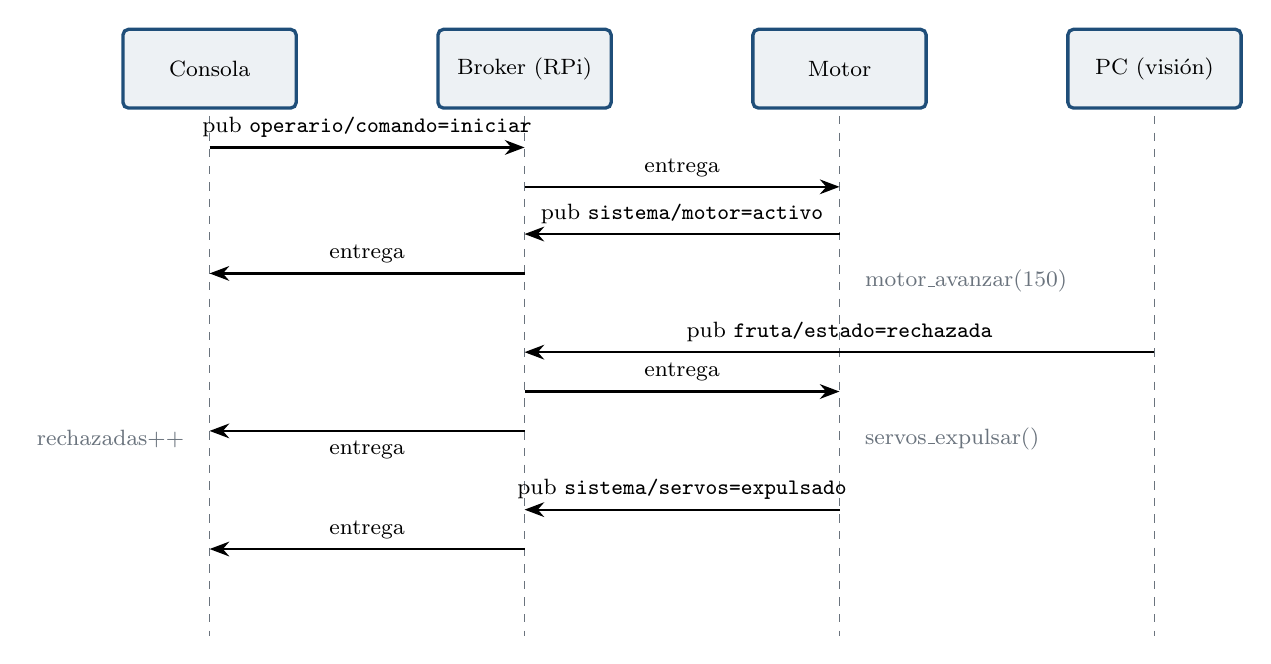
\begin{tikzpicture}[font=\footnotesize]
    % Lifelines
    \def\ytop{0} \def\ybot{-7.2}
    \foreach \x/\name in {0/Consola, 4/Broker (RPi), 8/Motor, 12/PC (visión)}{
      \node[bloque, minimum width=2.2cm] at (\x,\ytop) (h\x) {\name};
      \draw[griscmt, dashed] (\x,\ytop-0.6) -- (\x,\ybot);
    }
    % iniciar
    \draw[flecha] (0,-1.0) -- node[above]{pub \texttt{operario/comando=iniciar}} (4,-1.0);
    \draw[flecha] (4,-1.5) -- node[above]{entrega} (8,-1.5);
    \draw[flecha] (8,-2.1) -- node[above]{pub \texttt{sistema/motor=activo}} (4,-2.1);
    \draw[flecha] (4,-2.6) -- node[above]{entrega} (0,-2.6);
    \node[right, griscmt] at (8.2,-2.7) {motor\_avanzar(150)};
    % rechazada
    \draw[flecha] (12,-3.6) -- node[above]{pub \texttt{fruta/estado=rechazada}} (4,-3.6);
    \draw[flecha] (4,-4.1) -- node[above]{entrega} (8,-4.1);
    \draw[flecha] (4,-4.6) -- node[below]{entrega} (0,-4.6);
    \node[right, griscmt] at (8.2,-4.7) {servos\_expulsar()};
    \node[left, griscmt] at (-0.2,-4.7) {rechazadas++};
    \draw[flecha] (8,-5.6) -- node[above]{pub \texttt{sistema/servos=expulsado}} (4,-5.6);
    \draw[flecha] (4,-6.1) -- node[above]{entrega} (0,-6.1);
  \end{tikzpicture}
  \caption{Diagrama de secuencia MQTT para el arranque (comando del operario) y para un fruto rechazado. El broker desacopla a los nodos y replica cada mensaje a los suscriptores.}
  \label{fig:seq}
\end{figure}

% ====================================================================
\section{Diseño del firmware embebido}
\label{sec:firmware}
% ====================================================================

El firmware se desarrolla en C sobre ESP-IDF con un diseño modular. El nodo Motor separa responsabilidades en \texttt{config.h} (pines, red, tópicos), \texttt{motor}, \texttt{servos}, \texttt{mqtt\_handler} y \texttt{wifi\_manager}; el nodo Consola concentra OLED, botones y MQTT con tareas FreeRTOS dedicadas.

\subsection{Pinout del nodo ESP32 Motor}
La Tabla~\ref{tab:pinmotor} detalla la asignación de pines del nodo Motor, derivada de \texttt{config.h} y del cableado del BTS7960 y los servomotores.

\begin{table}[H]
\centering
\caption{Pinout del ESP32 Motor (driver BTS7960 + servomotores MG996R).}
\label{tab:pinmotor}
\footnotesize
\begin{tabular}{@{}lllc@{}}
\toprule
\textbf{GPIO} & \textbf{Señal} & \textbf{Destino} & \textbf{Dir.} \\
\midrule
25 & \texttt{RPWM} (PWM adelante) & BTS7960 RPWM & salida \\
26 & \texttt{LPWM} (PWM atrás) & BTS7960 LPWM & salida \\
32 & \texttt{R\_EN} (habilita der.) & BTS7960 R\_EN & salida \\
33 & \texttt{L\_EN} (habilita izq.) & BTS7960 L\_EN & salida \\
4 & PWM Servo 1 & Servomotor 1 (50\,Hz) & salida \\
5 & PWM Servo 2 & Servomotor 2 (50\,Hz) & salida \\
5V/GND & Alimentación lógica & BTS7960, servos & --- \\
\bottomrule
\end{tabular}
\end{table}

\subsection{Pinout del nodo ESP32 Consola}
La Tabla~\ref{tab:pinconsola} detalla los pines del nodo Consola (OLED I\textsuperscript{2}C, botones con \emph{pull-up} interno).

\begin{table}[H]
\centering
\caption{Pinout del ESP32 Consola (OLED I\textsuperscript{2}C, botones).}
\label{tab:pinconsola}
\footnotesize
\begin{tabular}{@{}lllc@{}}
\toprule
\textbf{GPIO} & \textbf{Señal} & \textbf{Destino} & \textbf{Dir.} \\
\midrule
21 & \texttt{SDA} (I\textsuperscript{2}C) & OLED (SSD1306 @ 0x3C) & E/S \\
22 & \texttt{SCL} (I\textsuperscript{2}C) & OLED (SSD1306 @ 0x3C) & salida \\
14 & Botón INICIAR & a GND (pull-up int.) & entrada \\
27 & Botón DETENER & a GND (pull-up int.) & entrada \\
26 & Botón PANTALLA & a GND (pull-up int.) & entrada \\
25 & Botón RESET & a GND (pull-up int.) & entrada \\
\bottomrule
\end{tabular}
\end{table}

\subsection{Consumo eléctrico de la consola portátil}
La consola está alimentada íntegramente desde una powerbank 12000\,mAh (capacidad nominal 12\,Wh @ 5V). En la Tabla~\ref{tab:consumo} se desglosa el consumo de cada componente y el tiempo de autonomía estimado.

\begin{table}[H]
\centering
\caption{Presupuesto de consumo eléctrico de la consola portátil.}
\label{tab:consumo}
\footnotesize
\begin{tabular}{@{}llccccl@{}}
\toprule
\textbf{Componente} & \textbf{Tipo} & \textbf{Voltaje} & \textbf{Corriente} & \textbf{Potencia} & \textbf{Duty} & \textbf{Notas} \\
\midrule
ESP32 (WiFi + core) & MCU & 3.3\,V & 80\,mA & 0.26\,W & 100\,\% & WiFi activo \\
OLED 128x64 & Display & 3.3\,V & 20\,mA & 0.07\,W & 100\,\% & Brillo normal \\
Botones (pull-ups) & Digital & 3.3\,V & 5\,mA & 0.02\,W & 100\,\% & 4 resistencias 10\,k \\
\midrule
\textbf{Total ESP32} & & & \textbf{105\,mA} & \textbf{0.35\,W} & & \\
\midrule
DC-DC Regulador & Boost 5V→3.3V & 5\,V & 63\,mA & 0.32\,W & 91\,\% & Eficiencia típica \\
\midrule
\textbf{Consumo Total} & & \textbf{5V} & \textbf{168\,mA} & \textbf{0.84\,W} & & \\
\midrule
\multicolumn{7}{c}{\textit{Autonomía con powerbank 12000\,mAh @ 5V nominal:}} \\
\multicolumn{7}{c}{\textit{Tiempo = 12000\,mAh / 168\,mA $\approx$ 71 horas (continuo)}} \\
\multicolumn{7}{c}{\textit{Operación típica ($\sim$8 horas/turno): Múltiples turnos sin recarga}} \\
\bottomrule
\end{tabular}
\end{table}

En la práctica, el consumo puede variar: modo profundo (light sleep) reduce a $\sim$10\,mA; actividad de botones es esporádica. La powerbank ofrece \textbf{autonomía de 2--3 días de operación típica} (8 horas/día).

\subsection{Concurrencia con FreeRTOS: disparo no bloqueante de servomotores}
El patrón embebido más relevante del proyecto resuelve RF-04. Cuando llega \texttt{fruta/estado=rechazada}, el \emph{callback} de MQTT \textbf{no} gira los servomotores directamente (eso lo bloquearía 350\,ms), sino que \emph{notifica} a una tarea dedicada mediante \texttt{xTaskNotifyGive}; la tarea mueve los servos, espera con \texttt{vTaskDelay} y publica la confirmación, todo sin congelar el hilo de red. El Código~\ref{lst:servos} muestra esta tarea.

\begin{lstlisting}[style=C, caption={Tarea FreeRTOS de los servomotores: espera una notificación, gira a 180°, retorna a neutral y confirma por MQTT, sin bloquear el hilo del broker.}, label={lst:servos}]
static void tarea_servos_expulsion(void *arg) {
    while (1) {
        // Bloquea aquí hasta recibir xTaskNotifyGive() desde el callback MQTT
        ulTaskNotifyTake(pdTRUE, portMAX_DELAY);

        ESP_LOGI(TAG, ">>> Disparando servomotores a 180 grados");
        servo_set_angle(1, 180);    // Servo 1 abre (180°)
        servo_set_angle(2, 180);    // Servo 2 abre (180°)
        
        vTaskDelay(pdMS_TO_TICKS(300));      // Mantener 300 ms
        
        servo_set_angle(1, 90);     // Servo 1 retorna a neutral (90°)
        servo_set_angle(2, 90);     // Servo 2 retorna a neutral (90°)
        
        vTaskDelay(pdMS_TO_TICKS(50));       // Estabilización

        ESP_LOGI(TAG, ">>> Servomotores retornados a neutral");

        if (cliente_mqtt)
            esp_mqtt_client_publish(cliente_mqtt, TOPIC_SERVOS, "expulsado", 0, 1, 0);
    }
}
\end{lstlisting}

El \emph{callback} de MQTT del nodo Motor interpreta los tópicos suscritos y solo dispara cuando el sistema está activo, como muestra el Código~\ref{lst:mqtt}.

\begin{lstlisting}[style=C, caption={Manejo de eventos MQTT en el nodo Motor (caso de datos recibidos con servomotores).}, label={lst:mqtt}]
if (strcmp(topic, TOPIC_COMANDO) == 0) {
    if (strcmp(data, "iniciar") == 0) {
        sistema_activo = true;  motor_avanzar(MOTOR_VEL_NORMAL);
        esp_mqtt_client_publish(client, TOPIC_MOTOR, "activo", 0, 1, 0);
    } else if (strcmp(data, "detener") == 0) {
        sistema_activo = false; motor_detener();
        esp_mqtt_client_publish(client, TOPIC_MOTOR, "detenido", 0, 1, 0);
    }
}
else if (strcmp(topic, TOPIC_FRUTA) == 0 && sistema_activo) {
    if (strcmp(data, "rechazada") == 0)
        xTaskNotifyGive(tarea_servos_handle);   // NOTIFICA a la tarea, no bloquea
}
\end{lstlisting}

\subsection{Máquinas de estados finitos (FSM) actualizadas}

El comportamiento de cada nodo se modela como una máquina de estados finitos. La Figura~\ref{fig:fsmmotor} presenta la FSM del nodo Motor actualizada con servomotores: tras el arranque conecta WiFi y MQTT, y alterna entre \texttt{DETENIDO} y \texttt{ACTIVO} según los comandos; en \texttt{ACTIVO}, un veredicto \texttt{rechazada} dispara los servomotores.

\begin{figure}[H]
  \centering
  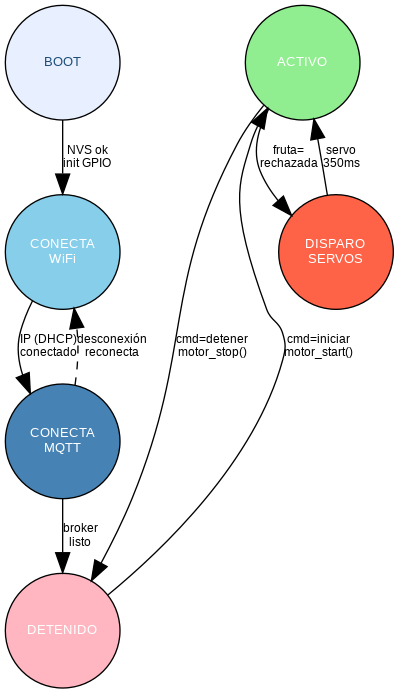
\includegraphics[width=0.85\textwidth]{./Figuras/fsm_motor_servos.png}
  \caption{FSM del nodo ESP32 Motor actualizada con servomotores MG996R. El estado \texttt{DISPARO SERVOS} se ejecuta en una tarea FreeRTOS separada (no bloqueante, duración total 350\,ms).}
  \label{fig:fsmmotor}
\end{figure}

La Figura~\ref{fig:fsmconsola} muestra la FSM de navegación de pantallas de la consola: el botón PANTALLA rota entre \texttt{CONTADORES}, \texttt{DIAGNÓSTICO} y \texttt{ALERTA}; tres rechazos consecutivos fuerzan el salto a \texttt{ALERTA} y lo muestran en pantalla OLED; el botón RESET limpia contadores y alerta.

\begin{figure}[H]
  \centering
  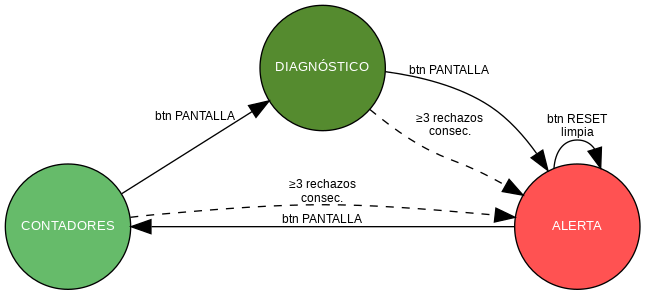
\includegraphics[width=0.85\textwidth]{./Figuras/fsm_consola.png}
  \caption{FSM de pantallas de la consola OLED. La transición forzada a \texttt{ALERTA} se dispara con tres rechazos consecutivos.}
  \label{fig:fsmconsola}
\end{figure}

% ====================================================================
\section{Caracterización y gráficas de respuesta}
\label{sec:respuestas}
% ====================================================================

\subsection{Señal PWM del motor}
El periférico LEDC genera la señal PWM a \SI{10}{\kilo\hertz} sobre \texttt{RPWM} (GPIO25). Con \texttt{MOTOR\_VEL\_NORMAL=150} sobre 255, el ciclo de trabajo es del 58.8\,\%, como se observa en la Figura~\ref{fig:pwm}. La Figura~\ref{fig:ledc} muestra la relación lineal entre el valor de \emph{duty} (8 bits) y la tensión media aplicada al motor, y el punto de operación elegido.

\begin{figure}[H]
  \centering
  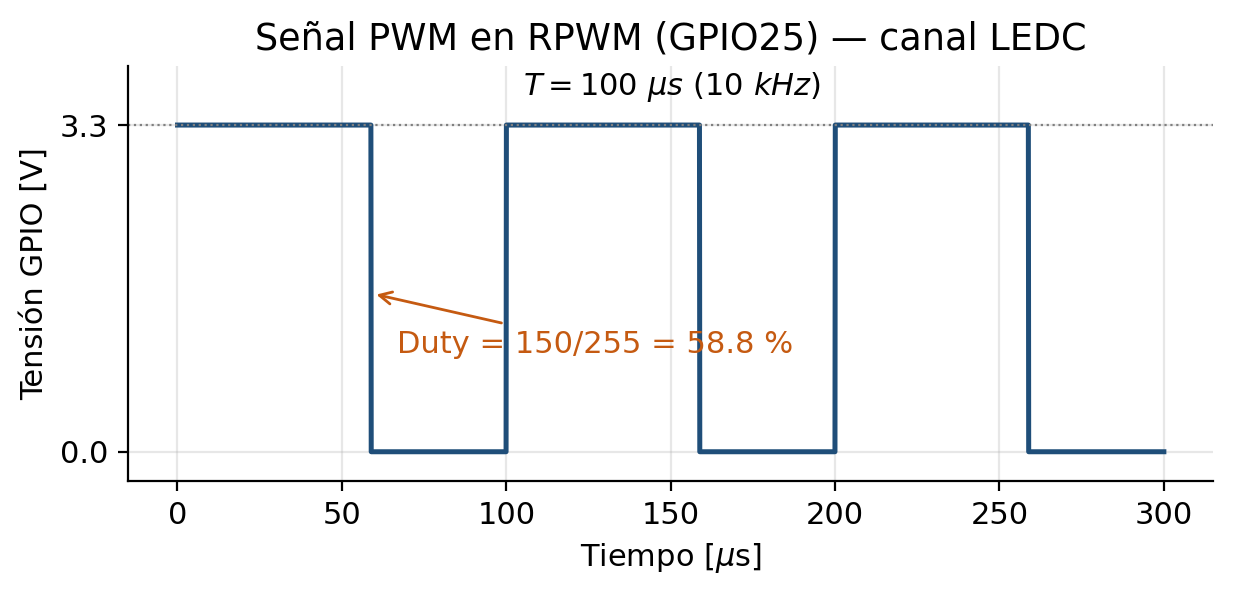
\includegraphics[width=0.82\textwidth]{./Figuras/pwm_10khz.png}
  \caption{Señal PWM a 10 kHz en GPIO25 con ciclo de trabajo de 150/255 (58.8\,\%). Período de \SI{100}{\micro\second}.}
  \label{fig:pwm}
\end{figure}

\begin{figure}[H]
  \centering
  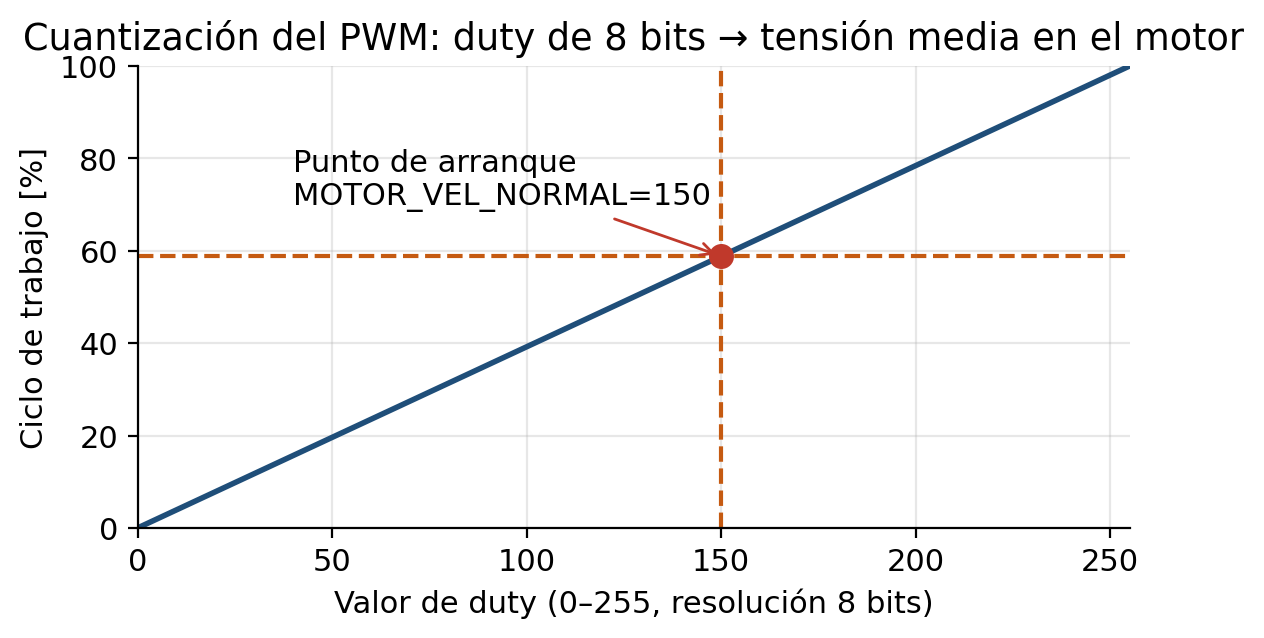
\includegraphics[width=0.72\textwidth]{./Figuras/ledc_duty.png}
  \caption{Cuantización del PWM: el \emph{duty} de 8 bits se mapea linealmente a la tensión media en el motor. En rojo, el punto de arranque (\emph{duty}=150).}
  \label{fig:ledc}
\end{figure}

La Figura~\ref{fig:pwm} es una representación a partir de los parámetros de configuración; en la defensa debe acompañarse de una \textbf{captura real de osciloscopio} sobre GPIO25 (ver Figura~\ref{fig:osc}).

\begin{figure}[H]
  \centering
  \fotopendiente[5.5cm]{Captura de osciloscopio de la señal PWM en GPIO25 (medir frecuencia $\approx$10 kHz y ciclo de trabajo).}
  \caption{Captura real de osciloscopio de la señal PWM (a incorporar).}
  \label{fig:osc}
\end{figure}

\subsection{Cronograma del disparo de servomotores}
La Figura~\ref{fig:cronoval} muestra la temporización del disparo no bloqueante: el evento MQTT \texttt{rechazada} provoca el giro de los servomotores (GPIO4, GPIO5) desde 90° a 180° durante \texttt{SERVO\_MS=300\,ms}; los servos actúan mecánicamente y, al retornar a neutral, el nodo publica \texttt{sistema/servos=expulsado}.

\begin{figure}[H]
  \centering
  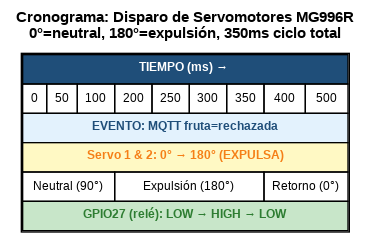
\includegraphics[width=0.92\textwidth]{./Figuras/cronograma_servos.png}
  \caption{Cronograma del disparo de servomotores gestionado por la tarea FreeRTOS dedicada. Incluye rampas de giro y estabilización.}
  \label{fig:cronoval}
\end{figure}

\subsection{Presupuesto de latencia extremo a extremo}
La Figura~\ref{fig:lat} descompone el tiempo total desde la captura hasta la expulsión. La etapa dominante es la inferencia de visión en la PC; las etapas de red y reacción embebida suman pocas decenas de milisegundos, de modo que el total se mantiene holgadamente por debajo de los 2\,s (RNF-01) y determina la velocidad máxima admisible de la banda.

\begin{figure}[H]
  \centering
  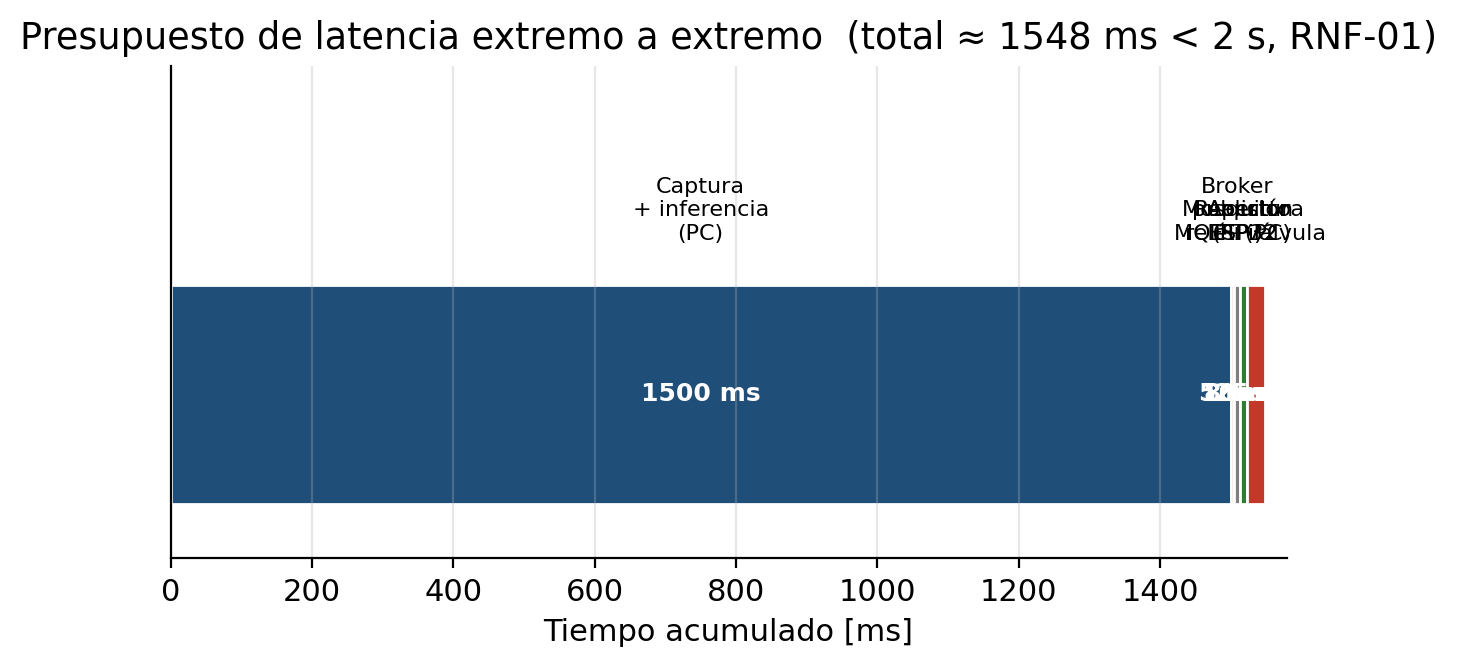
\includegraphics[width=0.92\textwidth]{./Figuras/latencia_e2e.png}
  \caption{Presupuesto de latencia extremo a extremo (valores típicos/de especificación). La inferencia domina; la cadena MQTT + reacción embebida es despreciable frente a ella.}
  \label{fig:lat}
\end{figure}

% ====================================================================
\section{Aplicación real: producción de tomate en Tarija}
\label{sec:tarija}
% ====================================================================

El fin último de la cinta es servir como herramienta de control de calidad poscosecha accesible a pequeños productores de tomate. Tarija reúne condiciones idóneas: pese a ser el departamento más pequeño de Bolivia, dispone de unas 189.268 hectáreas con vocación productiva agrícola \cite{eldiario2026potencial}, y el tomate es uno de los cultivos relevantes de sus valles \cite{elpais2023aviles}.

\paragraph{Comunidad propuesta: Chocloca (municipio de Uriondo, Valle Central).} Se propone como caso de aplicación la comunidad de \textbf{Chocloca}, uno de los nueve distritos del municipio de Uriondo (provincia José María Avilés), a unos 25\,km al sur de la ciudad de Tarija, en el Valle Central. El municipio agrupa 53 comunidades campesinas, de las cuales más del 90\,\% se dedica a la agricultura, con el tomate entre sus principales cultivos junto a la vid, la papa y el morrón \cite{elpais2023aviles}. Chocloca pertenece a la cuenca del río Camacho, de clima templado (temperatura media diaria máxima cercana a 26\,°C y precipitación media anual en torno a 740\,mm) \cite{erazo2003totora,wiki_uriondo}, lo que favorece varias campañas hortícolas al año.

\paragraph{Por qué es un caso idóneo.} Varios factores hacen pertinente el prototipo en esta comunidad:
\begin{itemize}
  \item \textbf{Clasificación manual y pérdidas.} La selección del tomate se hace a mano; un fruto deteriorado no detectado contamina el resto del lote, generando pérdidas.
  \item \textbf{Vulnerabilidad de la oferta.} La producción de tomate en Tarija llegó a caer hasta un 60\,\% por sequías y heladas; en un contexto de oferta ajustada, reducir el descarte tiene impacto económico directo.
  \item \textbf{Contexto rural sin Internet.} La arquitectura del proyecto opera sobre una red WiFi local autónoma (RPi como Access Point) y una consola a batería; no requiere conectividad externa (RNF-05).
\end{itemize}

% ====================================================================
\section{Anexo: material gráfico a incorporar}
% ====================================================================

Las figuras generadas (diagrama de bloques, secuencia MQTT, FSMs y gráficas de respuesta) ya están incluidas. Para completar la memoria con evidencia del prototipo real, se recomienda incorporar las siguientes \textbf{fotografías/capturas}, guardándolas en \texttt{./Figuras/} y reemplazando los recuadros reservados:

\begin{enumerate}
  \item \textbf{Montaje general} de la banda con 3 cámaras, zona de visión y zona de desvío (vista lateral y cenital).
  \item \textbf{Nodo ESP32 Motor} cableado al BTS7960 y servomotores MG996R (mostrar tierra común).
  \item \textbf{Captura de osciloscopio} de la señal PWM en GPIO25 (Figura~\ref{fig:osc}): verificar 10\,kHz y \emph{duty} 58.8\,\%.
  \item \textbf{Consola portátil} encendida mostrando la pantalla OLED con contadores.
  \item \textbf{Monitor serial} del ESP32 mostrando ``IP obtenida'' y ``Conectado al broker''.
  \item \textbf{Secuencia de expulsión}: foto de los servomotores desviando un tomate rechazado.
  \item \textbf{Tomates reales} de la zona usados en la prueba (sanos y deteriorados), idealmente de Chocloca/Uriondo.
\end{enumerate}

% --- Bibliografía APA 7ma ---
\newpage
\printbibliography[heading=bibintoc, title={Referencias Bibliográficas}]

\end{document}
